% Unit 109 terjemahan Bahasa Indonesia dari chapter8.tex baris 454--759.
% Sumber: Methods of Algebra, Volume 2, commit
% 9a5803ff77dd3257484cb177f851a73770a59dd3 (CC BY 4.0).
% stable-unit-id: o014.aljabr2.chapter8.geometric-realization
% Cakupan: Bagian 8.4 lengkap tentang funktor realisasi geometris, termasuk
% funktor singular, teorema produk, homotopi simplisial, dan tanda shuffle;
% berhenti tepat sebelum Bagian 8.5 tentang korespondensi Dold--Kan.

% segment-id: o014.aljabr2.chapter8.geometric-realization.h001
\section{Funktor Realisasi Geometris}\label{sec:geom-realization}
\hypertarget{o014.aljabr2.chapter8.geometric-realization}{ }
% segment-id: o014.aljabr2.chapter8.geometric-realization.p001
Sekarang kita mulai membangun gambaran geometris tentang himpunan simplisial yang
diperkenalkan dalam \S\ref{sec:simplicial-set}. Kita mulai dengan simpleks-$n$
standar, untuk $n\in\Z_{\geq0}$. Tuliskan basis terurut standar dari
$\R^{n+1}$ sebagai $e_0,\ldots,e_n$. Definisikan
% segment-id: o014.aljabr2.chapter8.geometric-realization.q001
\[
|\Delta^n| := \left\{ (x_0, \ldots, x_n) \in (\R_{\geq 0})^{n+1} : \sum_{i=0}^n x_i = 1 \right\} \quad
\begin{tikzpicture}[baseline=(O)]
	\coordinate (O) at (0, 0);
	\draw[-Latex] (0, 0) -- (-0.7, -0.7) node[left] {$e_0$};
	\draw[-Latex] (0, 0) -- (1, 0) node[right] {$e_1$};
	\draw[-Latex] (0, 0) -- (0, 1) node [above] {$e_2$};
	\fill[color=gray, opacity=0.4] (-0.4, -0.4) -- (0.75, 0) -- (0, 0.75) --cycle;
	\node at (1, -0.7) {(kasus khusus $n=2$)};
\end{tikzpicture}
\]
Titik-titik sudutnya dilabeli $0,\ldots,n$ melalui $i\leftrightarrow e_i$.
Interiornya dilengkapi orientasi standar sedemikian sehingga
$e_1-e_0,\ldots,e_n-e_{n-1}$ memberikan basis terurut positif di setiap
titik.

% segment-id: o014.aljabr2.chapter8.geometric-realization.p002
Setiap pemetaan monoton $f:[m]\to[n]$ menginduksi pemetaan
% segment-id: o014.aljabr2.chapter8.geometric-realization.q002
\[\begin{tikzcd}[row sep=tiny]
	{|f|}: {|\Delta^m|} \arrow[r] & {|\Delta^n|} \\
	\sum_{i=0}^m y_i e_i \arrow[mapsto, r] & \sum_{i=0}^m y_i e_{f(i)}.
\end{tikzcd}\]
Jika $f$ tidak surjektif, citra $|f|$ terletak pada batas. Pembenaman
$|\mathrm{d}^i|:|\Delta^{n-1}|\to|\Delta^n|$ dapat digunakan untuk
membandingkan orientasi interior $|\Delta^{n-1}|$ dengan orientasi yang
diinduksi $|\Delta^n|$ pada batasnya. Perhitungan determinan standar
menunjukkan bahwa keduanya berbeda sebesar faktor $(-1)^i$. Gambar berikut
melukiskan kasus $n=2$.
% segment-id: o014.aljabr2.chapter8.geometric-realization.g001
\begin{center}
	\begin{tikzpicture}
		\coordinate (A) at (0, 0);
		\coordinate (B) at (2, 0);
		\coordinate (C) at (1, 1.2);
		\fill[color=gray, opacity=0.25] (A) -- (B) -- (C) --cycle;
		\draw[ultra thick] (A) -- (B) -- (C) -- (A);
		\node[shape=circle, inner sep=0.3em, fill=white, draw] at (A) {$0$};
		\node[shape=circle, inner sep=0.3em, fill=white, draw] at (B) {$1$};
		\node[shape=circle, inner sep=0.3em, fill=white, draw] at (C) {$2$};

		\draw ($(B) + (0.8, 0.8)$) node[shape=rectangle, inner sep=0.3em, draw, below] {$0$} -- ($(C) + (0.8, 0.8)$) node[shape=rectangle, inner sep=0.3em, draw, above] {$1$};
		\draw[-Latex] ($(C)!0.5!(B) + (0.7, 0.7)$) to[edge label={$\mathrm{d}^0$}, swap] ($(C)!0.5!(B) + (0.2, 0.2)$);

		\draw ($(A) + (-0.8, 0.8)$) node[shape=rectangle, inner sep=0.3em, draw, below left] {$0$} -- ($(C) + (-0.8, 0.8)$) node[shape=rectangle, inner sep=0.3em, draw, above right] {$1$};
		\draw[-Latex] ($(A)!0.5!(C) + (-0.7, 0.7)$) to[edge label={$\mathrm{d}^1$}] ($(A)!0.5!(C) + (-0.2, 0.2)$);

		\draw ($(A) + (0, -1.2)$) node[shape=rectangle, inner sep=0.3em, draw, left] {$0$} -- ($(B) + (0, -1.2)$) node[shape=rectangle, inner sep=0.3em, draw, right] {$1$};
		\draw[-Latex] ($(A)!0.5!(B) + (0, -1)$) to[edge label={$\mathrm{d}^2$}] ($(A)!0.5!(B) + (0, -0.3)$);

		\node at (5, 2) {Orientasi:};
		\node (U) at (6.5, 2) {$0$};
		\node (V) at (8.5, 2) {$1$};
		\draw[->] (U) -- (V);
		\node (X) at (6.5, 0) {$0$};
		\node (Y) at (8.5, 0) {$1$};
		\node (Z) at (7.5, 1.2) {$2$};
		\draw[->] (X) -- (Y);
		\draw[->] (Y) -- (Z);
		\draw[->] (Z) -- (X);
	\end{tikzpicture}
\end{center}

% segment-id: o014.aljabr2.chapter8.geometric-realization.p003
Dengan merangkum pembahasan di atas, kita memperoleh funktor
% segment-id: o014.aljabr2.chapter8.geometric-realization.q003
\begin{equation*}
	|\cdot|: \simpDelta \to \cate{Top} \quad
	\left\{\begin{array}{ll}
		\text{objek} & [n] \mapsto |\Delta^n| \\
		\text{morfisme} & f \mapsto |f| .
	\end{array}\right.
\end{equation*}
Kita hendak memperluasnya menjadi funktor
$\cate{sSet}\to\cate{Top}$. Ingat bahwa $\cate{Top}$ kokomplet.

% segment-id: o014.aljabr2.chapter8.geometric-realization.d001
\begin{definition}[Funktor realisasi geometris]
	\index{realisasi geometris@realisasi geometris (geometric realization)}
	\index[sym1]{X-realization@$\lvert X\rvert$}
	Funktor $|\cdot|:\cate{sSet}\to\cate{Top}$ didefinisikan sebagai berikut.
	Jika $X$ himpunan simplisial, maka
% segment-id: o014.aljabr2.chapter8.geometric-realization.q004
	\[ |X| := \varinjlim_{n, x} |\Delta^n|, \]
	dengan $n\in\Z_{\geq0}$ dan $x\in X_n$, atau secara ekuivalen, dengan
	$x$ suatu morfisme $\Delta^n\to X$. Pasangan data $(n,x)$ tersebut membentuk suatu
	kategori. Morfisme dari $(n,x)$ ke $(m,y)$ tidak lain adalah
	$f\in\Hom_{\simpDelta}([n],[m])$ yang membuat diagram
% segment-id: o014.aljabr2.chapter8.geometric-realization.q005
	\[\begin{tikzcd}[column sep=small]
		\Delta^n \arrow[rr, "f"] \arrow[rd, "x"'] & & \Delta^m \arrow[ld, "y"] \\
		& X &
	\end{tikzcd}\]
	komutatif; secara ekuivalen, $f^*:X_m\to X_n$ harus memenuhi
	$f^*(y)=x$.
\end{definition}

% segment-id: o014.aljabr2.chapter8.geometric-realization.p004
Untuk $m\geq0$ tertentu, kategori data
$(n,x:\Delta^n\to\Delta^m)$ memiliki objek terminal
$(m,\identity_{\Delta^m})$. Karena itu, realisasi geometris $\Delta^m$
secara kanonik diidentifikasi dengan $|\Delta^m|$ yang didefinisikan
sebelumnya. Dengan demikian, notasinya konsisten.

% segment-id: o014.aljabr2.chapter8.geometric-realization.r001
\begin{remark}\label{rem:simplicial-density}
	Untuk setiap himpunan simplisial $X$, terdapat isomorfisme kanonik
	$\varinjlim_{n,x}\Delta^n\rightiso X$. Ini merupakan penerapan langsung
	Teorema Kerapatan~\ref{prop:Yoneda-density} pada kategori
	$\cate{sSet}=\simpDelta^{\wedge}$; pembaca dipersilakan memeriksanya.
\end{remark}

% segment-id: o014.aljabr2.chapter8.geometric-realization.r002
\begin{remark}
	Menurut Teorema~\ref{prop:Kan-limit}, realisasi geometris memberikan
	perluasan Kan kiri dari funktor $|\cdot|:\simpDelta\to\cate{Top}$ sepanjang
	$\simpDelta\to\cate{sSet}$; lihat Definisi~\ref{def:Kan-extension}.
	Dengan demikian, konstruksi ini sepenuhnya alami.
\end{remark}

% segment-id: o014.aljabr2.chapter8.geometric-realization.p005
Menurut konstruksi di atas, untuk setiap $n\in\Z_{\geq0}$ dan $x\in X_n$,
sifat universal $\varinjlim$ memberikan pemetaan kanonik
$i_{n,x}:|\Delta^n|\to|X|$ yang kompatibel ketika $(n,x)$ bervariasi.
Mengambil $\varinjlim$ dalam $\cate{Top}$ tidak lain adalah menempelkan
ruang-ruang topologis. Secara lebih konkret, realisasi geometris dapat
dituliskan sebagai ruang hasil bagi
% segment-id: o014.aljabr2.chapter8.geometric-realization.q006
\begin{equation}\label{eqn:geom-realization-quotient}
	|X| = \dfrac{\displaystyle\bigsqcup_{n \geq 0} X_n \times |\Delta^n| }{(f^*(y), t) \sim (y, |f|(t)) }, \quad
	\begin{tikzcd}[column sep=tiny]
		(f^*(y), t) \arrow[phantom, r, "\in" description] & X_n \arrow[phantom, r, "\times" description] & {|\Delta^n|} \arrow[d, "{|f|}"] & {[n]} \arrow[d, "f"] \\
		(y, {|f|}(t)) \arrow[phantom, r, "\in" description] & X_m \arrow[phantom, r, "\times" description] \arrow[u, "{f^*}"] & {|\Delta^m|} & {[m]}.
	\end{tikzcd}
\end{equation}

% segment-id: o014.aljabr2.chapter8.geometric-realization.p006
Sesuai intuisi geometris, himpunan simplisial $X$ dapat dibayangkan sebagai
suatu model ruang. Himpunan $X_0,X_1,\ldots$ merupakan kumpulan komponen
penyusun model itu: setiap elemen $X_n$ bersesuaian dengan, sekaligus melabeli,
satu salinan $|\Delta^n|$. Berbagai pemetaan
$f^*:X_m\to X_n$ berfungsi sebagai petunjuk perakitan yang menentukan cara
menempelkan salinan-salinan $|\Delta^n|$ tersebut.

% segment-id: o014.aljabr2.chapter8.geometric-realization.p007
Karena morfisme dalam $\simpDelta$ sudah dideskripsikan secara konkret,
relasi ekuivalensi dalam \eqref{eqn:geom-realization-quotient} dapat
dibangkitkan oleh dua jenis $f$ khusus.
% segment-id: o014.aljabr2.chapter8.geometric-realization.l001
\begin{itemize}
% segment-id: o014.aljabr2.chapter8.geometric-realization.i001
	\item Ambil $\mathrm{d}^i:[n-1]\hookrightarrow[n]$. Maka
	$|\mathrm{d}^i|$ menanamkan
	$\{d_i(x)\}\times|\Delta^{n-1}|$ ke dalam
	$\{x\}\times|\Delta^n|$. Jadi, pemetaan muka
	$d_i:X_n\to X_{n-1}$ melabeli muka ke-$i$ dari komponen berdimensi $n$
	(yang bersesuaian dengan $x$) sebagai $d_i(x)$, lalu penempelan dilakukan
	menurut label tersebut.

% segment-id: o014.aljabr2.chapter8.geometric-realization.i002
	\item Ambil $\mathrm{s}^j:[n+1]\twoheadrightarrow[n]$. Maka
	$|\mathrm{s}^j|$ ``memampatkan''
	$\{s_j(x)\}\times|\Delta^{n+1}|$ menjadi
	$\{x\}\times|\Delta^n|$. Jadi, pemetaan degenerasi
	$s_j:X_n\to X_{n+1}$ menentukan bagaimana suatu komponen berdimensi $n$
	(yang bersesuaian dengan $x$) menghasilkan komponen ``degenerat''
	berdimensi $n+1$, berlabel $s_j(x)$, yang dalam proses penempelan
	dimampatkan pada muka ke-$j$.
\end{itemize}
% segment-id: o014.aljabr2.chapter8.geometric-realization.p008
Karena itu, simpleks-$n$ degenerat (Definisi~\ref{def:simplex}) dapat
dihilangkan dari proses penempelan, tetapi informasi degenerasi tetap tidak
dapat diabaikan. Sebagai contoh, $d_i:X_n\to X_{n-1}$ sangat mungkin
memetakan simpleks nondegenerat ke simpleks degenerat.

% segment-id: o014.aljabr2.chapter8.geometric-realization.eg001
\begin{example}
	Sebagai ilustrasi, $\partial\Delta^n$ dalam
	Contoh~\ref{eg:boundary-horn} merealisasikan batas simpleks-$n$
	standar dalam pengertian intuitif, sedangkan tanduk $\Lambda^n_k$ diperoleh
	dengan membuang dari $\partial\Delta^n$ muka yang berhadapan dengan titik
	sudut ke-$k$. Berikut salah satu ilustrasinya:
% segment-id: o014.aljabr2.chapter8.geometric-realization.g002
	\begin{center}\begin{tikzpicture}
		\coordinate (A) at (0, 0);
		\coordinate (B) at (2, 0);
		\coordinate (C) at (1, 0.8);
		\coordinate (O) at (1, -1.5);

		\filldraw[thick, shading=radial, inner color=black!90, outer color=white] (A) node[left] {$1$} -- (C) node[above] {$3$} -- (B) node[right] {$2$} --($(O)!0.15!(C)$) --cycle;
		\draw (C) -- (O) node[below] {$0$};
		\filldraw[fill=white, thick] (A) -- (B) -- (O) --cycle;

		\node at ($(A) + (-1.5, -0.2)$) {$|\Lambda^3_0| =$};
	\end{tikzpicture}\end{center}
\end{example}

% segment-id: o014.aljabr2.chapter8.geometric-realization.eg002
\begin{example}\label{eg:cone-realization}
	\index{himpunan simplisial!kerucut@kerucut (cone)}
	Untuk setiap ruang topologis $\mathcal{X}$, definisikan kerucut di atasnya,
	$\Cone_{\mathrm{top}}(\mathcal{X})$, sebagai ruang yang
	diperoleh dengan mengerutkan subhimpunan tertutup
	$\mathcal{X}\times\{0\}$ dari $\mathcal{X}\times[0,1]$ menjadi satu
	titik. Secara visual,
% segment-id: o014.aljabr2.chapter8.geometric-realization.g003
	\[\Cone_{\mathrm{top}}(\mathcal{X}) = \; 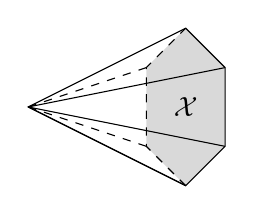
\begin{tikzpicture}[baseline=(P)]
		\coordinate (A) at (0, 1);
		\coordinate (B) at (0.5, 0.5);
		\coordinate (C) at (0.5, -0.5);
		\coordinate (D) at (0, -1);
		\coordinate (E) at (-0.5, -0.5);
		\coordinate (F) at (-0.5, 0.5);
		\coordinate (O) at (-2, 0);
		\coordinate (P) at (0, -0.1);	% For the baseline

		\fill[gray!50, opacity=0.6] (A) -- (B) -- (C) -- (D) -- (E) -- (F) --cycle;
		\draw (O) -- (A) -- (B) -- (C) -- (D) --cycle;
		\draw (O) -- (B);
		\draw (O) -- (C);
		\draw (O) -- (D);
		\draw[dashed] (D) -- (E) -- (F) -- (A);
		\draw[dashed] (O) -- (E);
		\draw[dashed] (O) -- (F);
		\node at (0, 0) {$\mathcal{X}$};
	\end{tikzpicture}\]
	Sebagai latihan sederhana, periksa bahwa
	$|X^{\lhd}|\simeq\Cone_{\mathrm{top}}(|X|)\simeq|X^{\rhd}|$. Ini
	menunjukkan bahwa kerucut dalam Definisi~\ref{def:cone-simplicial} memang
	layak disebut demikian; perbedaan antara kerucut kiri dan kanan hanya
	terletak pada orientasi.
\end{example}

% segment-id: o014.aljabr2.chapter8.geometric-realization.p009
Dengan menyajikan triangulasi ruang sebagai himpunan simplisial, banyak sifat
topologis penting dapat diekstraksi. Pendekatan ini secara tepat disebut
``topologi kombinatorial''. Pembahasan dan contoh lebih lanjut dapat dilihat
dalam \cite[Bab VI]{You}.

% segment-id: o014.aljabr2.chapter8.geometric-realization.d002
\begin{definition}[Funktor himpunan singular]
	\index[sym1]{Sing@$\mathrm{Sing}$}
	\index{himpunan singular@himpunan singular (singular set)}
	Untuk setiap ruang topologis $E$, definisikan himpunan simplisial
	$\mathrm{Sing}(E)$ melalui
% segment-id: o014.aljabr2.chapter8.geometric-realization.q007
	\[ \mathrm{Sing}(E)_n := \Hom_{\cate{Top}}(|\Delta^n|, E), \quad n \in \Z_{\geq 0}, \]
	dengan $d_i:\mathrm{Sing}(E)_n\to\mathrm{Sing}(E)_{n-1}$ (atau
	$s_j:\mathrm{Sing}(E)_n\to\mathrm{Sing}(E)_{n+1}$) diberikan oleh
	penarikan balik sepanjang
	$|\mathrm{d}^i|:|\Delta^{n-1}|\to|\Delta^n|$ (atau
	$|\mathrm{s}^j|:|\Delta^{n+1}|\to|\Delta^n|$). Objek ini disebut
	\emph{himpunan singular (simplisial)} yang bersesuaian dengan $E$.
	Konstruksi tersebut memberikan funktor
% segment-id: o014.aljabr2.chapter8.geometric-realization.q008
	\[ \mathrm{Sing}: \cate{Top} \to \cate{sSet}. \]
\end{definition}

% segment-id: o014.aljabr2.chapter8.geometric-realization.th001
\begin{theorem}\label{prop:geom-Sing-adjunction}
	Funktor realisasi geometris merupakan adjoin kiri dari funktor himpunan singular.
	Dengan kata lain, terdapat bijeksi alami
% segment-id: o014.aljabr2.chapter8.geometric-realization.q009
	\[\begin{tikzcd}[row sep=tiny]
		\Hom_{\cate{Top}}(|X|, E) \arrow[leftrightarrow, r, "1:1"] & \Hom_{\cate{sSet}}(X, \mathrm{Sing}(E)) \\
		\varphi \arrow[mapsto, r] & {\left[ X_n \xrightarrow{x \mapsto \varphi \circ i_{n, x}} \Hom_{\cate{Top}}(|\Delta^n|, E) \right]} \\
		\displaystyle\varinjlim_{(n, x)} \left( |\Delta^n| \xrightarrow{\psi_n(x)} E \right) & \psi = {\left[ \psi_n: X_n \to \Hom_{\cate{Top}}(|\Delta^n|, E) \right]}_{n \geq 0} , \arrow[mapsto, l]
	\end{tikzcd}\]
	dengan $X\in\Obj(\cate{sSet})$ dan $E\in\Obj(\cate{Top})$.
\end{theorem}
% segment-id: o014.aljabr2.chapter8.geometric-realization.pf001
\begin{proof}
	Ingat bahwa $|X|=\varinjlim_{n,x}|\Delta^n|$. Terdapat isomorfisme
	kanonik
% segment-id: o014.aljabr2.chapter8.geometric-realization.q010
	\begin{align*}
		\Hom_{\cate{Top}}\left( \varinjlim_{n, x} |\Delta^n| , E \right) & \rightiso \varprojlim_{n, x} \Hom_{\cate{Top}}(|\Delta^n|, E) = \varprojlim_{n, x} \mathrm{Sing}(E)_n \\
		& \rightiso \varprojlim_{n, x} \Hom_{\cate{sSet}}\left( \Delta^n, \mathrm{Sing}(E) \right) \\
		\varphi & \mapsto \left( \psi_n(x) := \varphi \circ i_{n, x} \right)_{n, x}.
	\end{align*}

	Setiap keluarga morfisme $(\psi_n(x))_{n,x}$ yang ditentukan oleh suatu
	$\psi:X\to\mathrm{Sing}(E)$ memenuhi kompatibilitas, yakni merupakan
	elemen $\varprojlim$ di ruas kanan rumus di atas. Bukti akan selesai jika
	kita menunjukkan bahwa memberikan morfisme $\psi$ sama artinya dengan memberikan
	keluarga morfisme yang kompatibel; tepat inilah yang dijamin oleh
	Catatan~\ref{rem:simplicial-density}.
\end{proof}

% segment-id: o014.aljabr2.chapter8.geometric-realization.r003
\begin{remark}
	Untuk kajian teori homotopi, kategori $\cate{CGHaus}$ yang disebutkan dalam
	\S\ref{sec:closed-monoidal} mungkin lebih nyaman daripada $\cate{Top}$.
	Karena funktor inklusi $\cate{CGHaus}\to\cate{Top}$ mempunyai adjoin kanan
	$k$, funktor tersebut mempertahankan $\varinjlim$. Selain itu,
	$|\Delta^n|$ adalah ruang Hausdorff yang dibangkitkan secara kompak. Maka,
	penempelan (atau pengambilan $\Hom$) dalam realisasi geometris (atau
	himpunan singular) dapat dilakukan di dalam $\cate{CGHaus}$\footnote{Perlu
	dijelaskan bahwa $\varinjlim$ yang dibahas memang ada dalam
	$\cate{CGHaus}$. Ini merupakan persoalan topologis; lihat
	\cite[III.1.8, III.2.1]{GZ67}.}. Dengan demikian, pasangan adjoin dalam
	Teorema~\ref{prop:geom-Sing-adjunction} berfaktor sebagai dua adjungsi, yang
	ditulis menggunakan notasi yang sama sebagai
% segment-id: o014.aljabr2.chapter8.geometric-realization.q011
	\[\begin{tikzcd}
		\cate{sSet} \arrow[shift left, r, "{|\cdot|}"] & \cate{CGHaus} \arrow[shift left, r, "\text{funktor inklusi}"] \arrow[shift left, l, "\mathrm{Sing}"] & \cate{Top} \arrow[shift left, l, "k"] .
	\end{tikzcd}\]
\end{remark}

% segment-id: o014.aljabr2.chapter8.geometric-realization.p010
Untuk sembarang dua himpunan simplisial $X$ dan $Y$, hasil kalinya
didefinisikan sebagai hasil kali suku demi suku:
% segment-id: o014.aljabr2.chapter8.geometric-realization.q012
\begin{gather*}
	(X \times Y)_n = X_n \times Y_n, \\
	d_i(x, y) = (d_i(x), d_i(y)), \\
	s_j(x, y) = (s_j(x), s_j(y)).
\end{gather*}
Ini sekaligus merupakan hasil kali kategoris dalam
$\cate{sSet}=\cate{Set}^{\simpDelta^{\opp}}$ dan konstruksi dalam
Definisi~\ref{def:monoidal-sObj} ketika kategori monoidal yang digunakan
adalah $(\cate{Set},\times)$. Walaupun kedua definisi ini berasal dari teori
kategori, hasil mendasar berikut menunjukkan bahwa keduanya juga mempunyai
makna geometris.

% segment-id: o014.aljabr2.chapter8.geometric-realization.th002
\begin{theorem}\label{prop:realization-product}
	Untuk himpunan simplisial $X$ dan $Y$, terdapat isomorfisme kanonik dalam
	$\cate{CGHaus}$
% segment-id: o014.aljabr2.chapter8.geometric-realization.q013
	\[ |X \times Y| \simeq |X| \times |Y|. \]
	Secara lebih umum, versi $|\cdot|$ yang bernilai dalam $\cate{CGHaus}$
	mempertahankan $\varprojlim$ hingga. Jika $X$ atau $Y$ hanya mempunyai
	hanya memiliki sejumlah hingga simpleks nondegenerat, maka
	$|X\times Y|\simeq|X|\times|Y|$ juga berlaku dalam $\cate{Top}$.
\end{theorem}

% segment-id: o014.aljabr2.chapter8.geometric-realization.p011
Bukti dalam keadaan umum cukup rumit; lihat \cite[Bab III]{GZ67} atau
\cite{Dri03}. Isomorfisme tersebut pada umumnya tidak berlaku bagi versi
realisasi geometris yang bernilai dalam $\cate{Top}$. Perhatikan bahwa syarat
yang diberikan oleh teorema untuk versi $\cate{Top}$ bukanlah syarat optimal.

% segment-id: o014.aljabr2.chapter8.geometric-realization.c001
\begin{corollary}
	Tuliskan $\cate{Grp}$ untuk kategori grup. Jika himpunan simplisial $X$
	dapat diperluas menjadi objek $\cate{sGrp}$, maka $|X|$ secara alami
	mempunyai struktur grup topologis. Hasil serupa berlaku bagi struktur
	aljabar lainnya.
\end{corollary}

% segment-id: o014.aljabr2.chapter8.geometric-realization.p012
Berdasarkan Teorema~\ref{prop:realization-product}, wajar untuk mendefinisikan
suatu homotopi dari $g$ ke $f$, bagi morfisme
$f,g:X\rightrightarrows Y$ dalam $\cate{sSet}$, sebagai morfisme
$H:X\times\Delta^1\to Y$ yang membuat diagram berikut komutatif:
% segment-id: o014.aljabr2.chapter8.geometric-realization.q014
\begin{equation}\label{eqn:simplicial-homotopy-prep}
	\begin{tikzcd}
		X \times \Delta^0 \arrow[d, "{\identity_X \times \mathrm{d}^0}"'] \arrow[r, "\sim"] & X \arrow[d, "f"] \\
		X \times \Delta^1 \arrow[r, "H" description] & Y \\
		X \times \Delta^0 \arrow[u, "{\identity_X \times \mathrm{d}^1}"] \arrow[r, "\sim"'] & X \arrow[u, "g"']
	\end{tikzcd}
\end{equation}

% segment-id: o014.aljabr2.chapter8.geometric-realization.p013
Sebagai kasus khusus, komposisi
$X\times\Delta^1\xrightarrow{\text{proyeksi}}X\xrightarrow{f}Y$
memberikan homotopi konstan dari $f$ ke dirinya sendiri. Namun, homotopi yang
didefinisikan dengan cara ini bukan relasi ekuivalensi: contoh sederhana
sudah menunjukkan bahwa sifat simetri tidak terpenuhi. Dalam teori homotopi,
biasanya $Y$ disyaratkan mempunyai sifat tambahan, misalnya merupakan
kompleks Kan. Dalam keadaan tersebut, relasi homotopi memiliki
sifat-sifat yang diharapkan, sehingga grup homotopi, ekuivalensi lemah, dan
konsep-konsep lain dapat dikaji secara kombinatorial.

% segment-id: o014.aljabr2.chapter8.geometric-realization.p014
Walaupun buku ini tidak membuktikan
Teorema~\ref{prop:realization-product}, ada gunanya meninjau kasus khusus
sederhana $X=\Delta^p$ dan $Y=\Delta^q$. Sebagai contoh,
bagaimana simpleks-simpleks nondegenerat dari
$\Delta^p\times\Delta^q$ dapat diklasifikasikan? Jawabannya bukan hanya
membantu memahami realisasi geometris hasil kali; konstruksi terkait juga
akan diperlukan kemudian.

% segment-id: o014.aljabr2.chapter8.geometric-realization.p015
Pertama, hasil kali dua himpunan terurut parsial $S_1$ dan $S_2$ menjadi
himpunan terurut parsial melalui
$(a_1,a_2)\leq(b_1,b_2)$ jika dan hanya jika
$a_1\leq b_1$ dan $a_2\leq b_2$. Ini juga sama dengan mengambil hasil kali
kategori-kategori yang bersesuaian dengannya.

% segment-id: o014.aljabr2.chapter8.geometric-realization.d003
\begin{definition}\label{def:pq-shuffle}
	\index{shuffle p-q@shuffle $(p, q)$ ($(p, q)$-shuffle)}
	Misalkan $p,q\in\Z_{\geq0}$. Suatu \emph{shuffle-$(p,q)$} adalah pemetaan
	monoton injektif $\sigma:[p+q]\to[p]\times[q]$.
\end{definition}

% segment-id: o014.aljabr2.chapter8.geometric-realization.p016
Untuk setiap $n\in\Z_{\geq0}$, menentukan pemetaan monoton
$\sigma:[n]\to[p]\times[q]$ setara dengan menentukan sepasang pemetaan
monoton $\sigma_-:[n]\to[p]$ dan $\sigma_+:[n]\to[q]$. Ini juga setara
dengan menentukan suatu simpleks-$n$ dari $\Delta^p\times\Delta^q$.
Syarat bahwa $\sigma$ injektif setara dengan syarat bahwa lintasan
$i\mapsto(\sigma_-(i),\sigma_+(i))$ tidak pernah diam, untuk
$i=0,\ldots,n$. Jika $n=p+q$, keadaan ini dapat digambarkan sebagai berikut:
% segment-id: o014.aljabr2.chapter8.geometric-realization.q015
\begin{equation}\label{eqn:pq-shuffle-diag}
	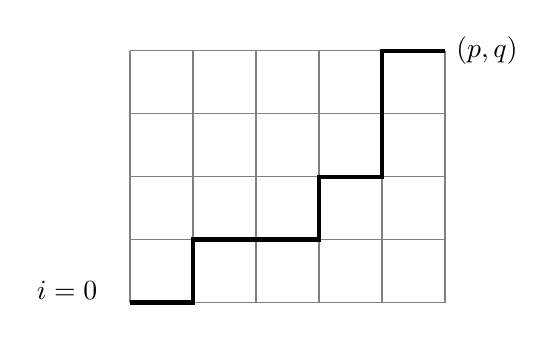
\begin{tikzpicture}[scale=0.8, baseline=(O)]
		\draw[thin, gray] (0, 0) grid (5, 4);
		\node at (-1, 0.2) {$i=0$};
		\draw[ultra thick] (0, 0) -- (1, 0) -- (1, 1) -- (2, 1) -- (3, 1) -- (3, 2) -- (4, 2) -- (4, 3) -- (4, 4) -- (5, 4) node[right] {$(p, q)$};
		\coordinate (O) at (0, 2);
	\end{tikzpicture}
	\quad
	\text{tepat $p+q$ langkah.}
\end{equation}
Jadi, untuk shuffle-$(p,q)$ $\sigma$, definisikan
% segment-id: o014.aljabr2.chapter8.geometric-realization.q016
\begin{align*}
	I_\pm & := \left\{ 1 \leq i \leq p+q : \sigma_\pm(i-1) < \sigma_\pm(i) \right\} \\
	& = \left\{ 1 \leq i \leq p+q : \sigma_\pm(i-1) = \sigma_\pm(i) - 1 \right\} \\
	& = \left\{ 1 \leq i \leq p+q: \sigma_\mp(i-1) = \sigma_\mp(i) \right\},
\end{align*}
dengan $I_+\sqcup I_-=\{1,\ldots,p+q\}$. Subhimpunan $I_+$ (atau $I_-$)
bersesuaian dengan bagian lintasan yang bergerak ke atas (atau ke kanan)
dalam \eqref{eqn:pq-shuffle-diag}. Dengan demikian, shuffle-$(p,q)$ juga
dapat dipandang sebagai suatu urutan yang terdiri atas $p$ simbol
$\rightarrow$ dan $q$ simbol $\uparrow$; jumlahnya
$\binom{p+q}{p}$. Pengamatan ini sekaligus menunjukkan bahwa $\sigma_+$ dan
$\sigma_-$ dari suatu shuffle-$(p,q)$ adalah pemetaan monoton surjektif.

% segment-id: o014.aljabr2.chapter8.geometric-realization.pr001
\begin{proposition}
	Misalkan $p,q\in\Z_{\geq0}$. Tinjau suatu simpleks-$n$ dari
	$\Delta^p\times\Delta^q$, yakni pemetaan monoton
	$\sigma:[n]\to[p]\times[q]$. Tetapkan
	$(p_i,q_i):=\sigma(i)$ dan
	$(p',q'):=(p_n-p_0,q_n-q_0)$. Maka $\sigma$ nondegenerat jika dan hanya
	jika syarat-syarat berikut terpenuhi:
	\begin{itemize}
		\item $p'+q'=n$;
		\item $\sigma$ merupakan komposisi suatu shuffle-$(p',q')$
		$\sigma':[n]\to[p']\times[q']$ dengan suatu injeksi monoton
		$[p']\times[q']\hookrightarrow[p]\times[q]$ berbentuk $f\times g$.
	\end{itemize}
\end{proposition}
% segment-id: o014.aljabr2.chapter8.geometric-realization.pf002
\begin{proof}
	Identifikasikan $\sigma$ dengan pasangan pemetaan monoton
	$(\sigma_-,\sigma_+)$. Tinjau lintasan $i\mapsto(p_i,q_i)$ seperti dalam
	Gambar~\eqref{eqn:pq-shuffle-diag}. Syarat bahwa $\sigma$ nondegenerat
	setara dengan syarat bahwa lintasan itu tidak pernah diam. Selebihnya
	jelas.
\end{proof}

% segment-id: o014.aljabr2.chapter8.geometric-realization.p017
Berdasarkan deskripsi simpleks nondegenerat tersebut, pembaca dapat
memahami secara geometris
$|\Delta^p\times\Delta^q|\simeq|\Delta^p|\times|\Delta^q|$ bagi
$(p,q)=(1,1)$ dan $(2,1)$. Sebagai contoh, gambar berikut memperlihatkan
triangulasi $|\Delta^2|\times|\Delta^1|$ menjadi tiga tetrahedron, yang
bersesuaian dengan $3=\binom{3}{2}$ shuffle-$(2,1)$.

% segment-id: o014.aljabr2.chapter8.geometric-realization.g004
\begin{center}\begin{tikzpicture}[yscale=0.8]
	\coordinate (A) at (0, 0);
	\coordinate (B) at (2.2, 0.5);
	\coordinate (C) at (0.8, -0.5);
	\coordinate (P) at ($(A) + (0, -3)$);
	\coordinate (Q) at ($(B) + (0, -3)$);
	\coordinate (R) at ($(C) + (0, -3)$);

	\draw ($(A) + (-5, -0.3)$) -- ($(B) + (-5, -0.3)$) -- ($(Q) + (-5, -0.3)$) -- ($(R) + (-5, -0.3)$) -- ($(P) + (-5, -0.3)$) --cycle;
	\draw ($(A) + (-5, -0.3)$) -- ($(C) + (-5, -0.3)$) -- ($(B) + (-5, -0.3)$);
	\draw ($(C) + (-5, -0.3)$) -- ($(R) + (-5, -0.3)$);
	\draw[dashed] ($(P) + (-5, -0.3)$) -- ($(Q) + (-5, -0.3)$);

	\draw[-Latex] ($(B)!0.5!(Q) + (-4.5, -0.5)$) -- ($(B)!0.5!(Q) + (-3, -0.5)$);

	\draw (A) -- (B) -- (C) --cycle;
	\draw (A) -- (P) -- (C);
	\draw (P) -- (B);

	\draw[fill=white] ($(P) + (0.2, -1.2)$) -- ($(B) + (0.2, -1.2)$) -- ($(R) + (0.2, -1.2)$) --cycle;
	\draw[fill=white] ($(R) + (0.2, -1.2)$) -- ($(Q) + (0.2, -1.2)$) -- ($(B) + (0.2, -1.2)$) --cycle;

	\draw[fill=white] ($(P) + (0.1, -0.6)$) -- ($(R) + (0.1, -0.6)$) -- ($(C) + (0.1, -0.6)$) --cycle;
	\draw[fill=white] ($(R) + (0.1, -0.6)$) -- ($(B) + (0.1, -0.6)$) -- ($(C) + (0.1, -0.6)$) --cycle;
\end{tikzpicture}\end{center}

% segment-id: o014.aljabr2.chapter8.geometric-realization.d004
\begin{definition}\label{def:pq-shuffle-sgn}
	Misalkan $\sigma$ suatu shuffle-$(p,q)$. Tandanya didefinisikan sebagai
% segment-id: o014.aljabr2.chapter8.geometric-realization.q017
	\[ \sgn(\sigma) := (-1)^{|I_\sigma|}, \quad I_\sigma := \left\{ (i, j) \in I_- \times I_+ : i > j \right\}. \]
\end{definition}

% segment-id: o014.aljabr2.chapter8.geometric-realization.p018
Jika $\sigma$ dipandang sebagai urutan $p$ simbol $\rightarrow$ dan $q$
simbol $\uparrow$, maka $I_\sigma$ tepat merupakan himpunan semua pasangan
$(j,i)$, dengan $j<i$, yang muncul dalam urutan ``terbalik''
$(\uparrow,\rightarrow)$. Suatu latihan kombinatorial sederhana menunjukkan
bahwa terdapat tepat satu $\tau\in\mathfrak{S}_{p+q}$ yang menyusun kembali
urutan itu menjadi
$\rightarrow\cdots\rightarrow\uparrow\cdots\uparrow$ tanpa mengubah urutan
internal dalam $I_+$ maupun $I_-$. Definisi~\ref{def:pq-shuffle-sgn} dengan
demikian sama artinya dengan $\sgn(\sigma)=\sgn(\tau)$.

% segment-id: o014.aljabr2.chapter8.geometric-realization.p019
Untuk shuffle-$(p,q)$ $\sigma$, menukar peran $\sigma_-$ dan $\sigma_+$
memberikan shuffle-$(q,p)$ $\sigma'$. Penafsiran di atas dan argumen
kombinatorial dasar memberikan
% segment-id: o014.aljabr2.chapter8.geometric-realization.q018
\begin{equation}\label{eqn:shuffle-sign-0}
	\sgn(\sigma) = (-1)^{pq} \sgn(\sigma').
\end{equation}

% segment-id: o014.aljabr2.chapter8.geometric-realization.p020
Dengan asas yang sama, definisikan shuffle-$(p,q,r)$ sebagai injeksi monoton
$\sigma=(\sigma_-,\sigma_0,\sigma_+):[p+q+r]\to[p]\times[q]\times[r]$,
atau, secara ekuivalen, pandang $\sigma$ sebagai suatu urutan simbol
$\rightarrow$, $\nearrow$, dan $\uparrow$. Definisikan
$\sgn(\sigma):=(-1)^{|I_\sigma|}$, dengan $I_\sigma$ terdiri atas semua
tripel indeks $k>j>i$ yang bersesuaian dengan permutasi ganjil dari
$(\rightarrow,\nearrow,\uparrow)$. Latihan kombinatorial standar yang sama
menunjukkan bahwa jika shuffle-$(p,q,r)$ $\sigma$ mempunyai faktorisasi
% segment-id: o014.aljabr2.chapter8.geometric-realization.q019
\[ [p+q+r] \xrightarrow{\sigma_1} [p+q] \times [r] \xrightarrow{\sigma_2 \times \identity_{[r]}} [p] \times [q] \times [r], \]
maka $\sigma_1$ merupakan shuffle-$(p+q,r)$, $\sigma_2$ merupakan
shuffle-$(p,q)$, dan
% segment-id: o014.aljabr2.chapter8.geometric-realization.q020
\begin{equation}\label{eqn:shuffle-sign-1}
	\sgn(\sigma) = \sgn(\sigma_1) \sgn(\sigma_2).
\end{equation}
Pernyataan serupa tentu berlaku bagi faktorisasi
$[p+q+r]\to[p]\times[q+r]\to[p]\times[q]\times[r]$.

% segment-id: o014.aljabr2.chapter8.geometric-realization.p021
Persamaan~\eqref{eqn:shuffle-sign-0} dan
\eqref{eqn:shuffle-sign-1} pada hakikatnya sepenuhnya kombinatorial;
verifikasi terperinci diserahkan sebagai latihan bab ini. Pengamatan tersebut
akan digunakan dalam \S\ref{sec:bisimplicial}.
